\documentclass[12pt, times new roman]{report}
\usepackage[utf8]{inputenc}
\usepackage{color}
\usepackage{listings}
\usepackage{float}
\usepackage{graphicx}

\definecolor{codegreen}{rgb}{0,0.6,0}
\definecolor{codegray}{rgb}{0.5,0.5,0.5}
\definecolor{codepurple}{rgb}{0.58,0,0.82}
\definecolor{backcolour}{rgb}{0.95,0.95,0.92}

\lstdefinestyle{mystyle}{
    backgroundcolor=\color{backcolour},   
    commentstyle=\color{codegreen},
    keywordstyle=\color{magenta},
    numberstyle=\tiny\color{codegray},
    stringstyle=\color{codepurple},
    basicstyle=\footnotesize,
    breakatwhitespace=false,         
    breaklines=true,                 
    captionpos=b,                    
    keepspaces=true,                 
    numbers=left,                    
    numbersep=5pt,                  
    showspaces=false,                
    showstringspaces=false,
    showtabs=false,                  
    tabsize=2,
    language=python
}

\lstset{style=mystyle}

\title{Tugas Pemrograman Chapter 4}
\author{Ariq rafi kusumah (1184076)}
\date{\today}

\begin{document}

\maketitle

\chapter{Teori}

\section{Apa itu fungsi file CVS,sejarah dan contoh}

\subsection{Fungsi File CVS}
\hspace{0.5cm}Format file csv Comma Separated Values yaitu suatu format data pada
basis data dimana setiap record yang dapat dipisahkan dengan menggunakan tanda koma (‘,’) atau juga bisa dengan menggunakan titik koma (‘;’)
sebagai tanda pemisah antara datu elemen dengan elemen yang lainnya.
Selain bahasa programnya yang sederhana, format ini juga dapat dibuka
dengan menggunakan berbagai text-editor seperti Notepad, Wordpad, dan
MS Excel.

\subsection{Sejarah file CVS}

\hspace{0.5cm}Nilai yang dipisahkan oleh koma adalah format data yang memberi tanggal lebih awal pada komputer pribadi lebih dari satu dekade: kompiler
IBM Fortran (level H extended) di bawah OS / 360 mendukungnya pada
tahun 1972. Input / output yang diarahkan oleh daftar (”bentuk bebas”)
didefinisikan dalam FORTRAN 77, disetujui pada tahun 1978. Input yang
diarahkan daftar menggunakan koma atau spasi untuk pembatas, sehingga
string karakter yang tidak dikutip tidak dapat mengandung koma atau
spasi.\\

Nama (nilai dipisahkan koma) dan singkatan (CSV) digunakan pada
tahun 1983. Manual untuk komputer Osborne Executive, yang menggabungkan SuperCalc spreadsheet, mendokumentasikan konvensi kutipan
CSV yang memungkinkan string berisi koma yang disematkan, tetapi manual tersebut tidak menentukan konvensi untuk menyematkan tanda kutip
dalam string yang dikutip. Daftar nilai yang dipisahkan koma lebih mudah untuk diketik (misalnya ke dalam kartu berlubang) daripada data
yang selaras dengan kolom tetap dan cenderung menghasilkan hasil yang
salah jika suatu nilai dilubangi satu kolom dari lokasi yang dituju.\\

Pada 2014 IETF menerbitkan RFC7111 yang menjelaskan aplikasi fragmen URI ke dokumen CSV. RFC7111 menentukan bagaimana rentang
baris, kolom, dan sel dapat dipilih dari dokumen CSV menggunakan indeks posisi. Pada 2015 W3C, dalam upaya meningkatkan CSV dengan
semantik formal, mempublikasikan draft rekomendasi pertama untuk standar metadata CSV, yang dimulai sebagai rekomendasi pada bulan Desember tahun yang sama.

\subsection{Contoh}

\lstinputlisting[language=Python]{src/contoh.csv}

\section{Aplikasi-aplikasi apa saja yang bisa menciptakan file CVS}
\begin{enumerate}
    \item Text Editor (Notepad, Wordpad, dll)
    \item Spreadsheet (Microsoft Excel)
\end{enumerate}

\section{Cara menulis dan membaca file CVS di excel atau spreadsheet}

\begin{enumerate}
    \item Pertama, Membuka Excle 
    \item Isikan Seperti di gambar ini :
    \begin{figure}[h]
        \centering
        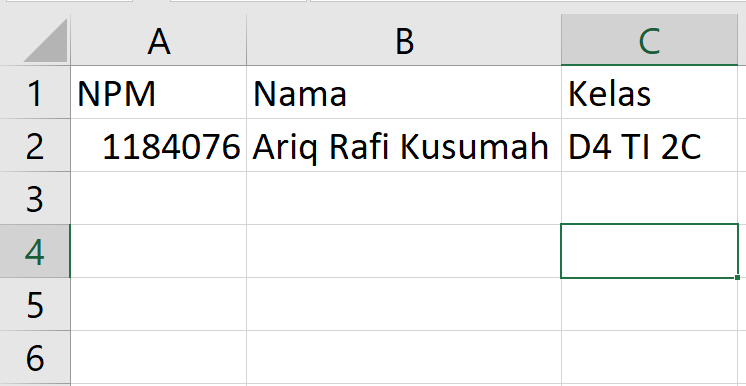
\includegraphics[scale=0.7]{figures/Make1.PNG}
        \caption{Mengisikan Kolom}
        \label{fig:my_label}
    \end{figure}
    \\
    \\
    \item Setelah Mengisi datanya, langsung ke tahap save file dengan format CVS.
    \begin{figure}[ht]
        \centering
        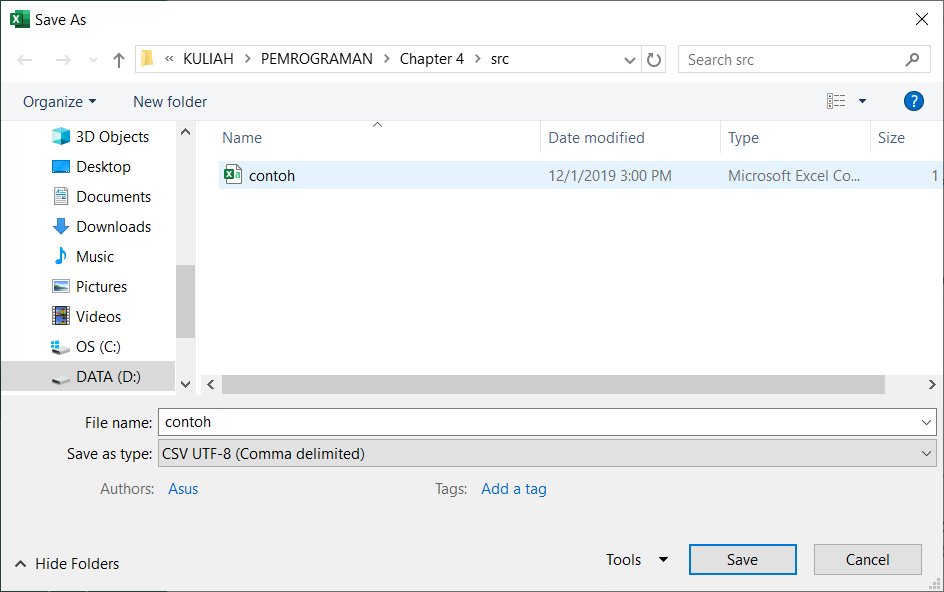
\includegraphics[scale=0.5]{figures/Make2.PNG}
        \caption{Save File Format}
        \label{fig:my_label}
    \end{figure}
    \item File CVS telah terbuat.
\end{enumerate}

\newpage

\section{Sejarah Library CVS}
\hspace{0.5cm}Format yang disebut CSV Comma Separated Values adalah format impor
dan ekspor paling umum untuk spreadsheet dan basis data. Format CSV digunakan selama bertahun-tahun sebelum upaya untuk menggambarkan format
dengan cara standar di RFC 4180. Kurangnya standar yang didefinisikan dengan baik berarti bahwa perbedaan halus sering ada dalam data yang diproduksi
dan dikonsumsi oleh aplikasi yang berbeda. Perbedaan-perbedaan ini dapat
membuatnya menjengkelkan untuk memproses file CSV dari berbagai sumber\\

Namun, sementara pembatas dan mengutip karakter bervariasi, format keseluruhan cukup mirip sehingga dimungkinkan untuk menulis satu modul yang
dapat secara efisien memanipulasi data seperti itu, menyembunyikan detail
membaca dan menulis data dari programmer. Modul csv mengimplementasikan
kelas untuk membaca dan menulis data tabular dalam format CSV.

\section{Sejarah Library Pandas}
\hspace{0.7cm}Pandas adalah toolkit yang powerfull sebagai alat analisis data dan struktur
untuk bahasa pemrograman Python. Dengan menggunakan pandas kita dapat
mengolah data dengan mudah, salah satu fiturnya adalah Dataframe. Dengan
adanya fitur dataframe kita dapat membaca sebuah file dan menjadikannya tabble serta juga dapat mengolah suatu data dengan menggunakan operasi seperti
join, distinct, group by, agregasi, dan lain-lain yang terdapat pada SQL. Banyak
format file yang dapat dibaca menggunakan Pandas, seperti file .txt, .csv, .tsv
dan lainnya. Agar lebih jelas mari kita mencobanya secara langsung.

\section{Fungsi-fungsi yang terdapat di library csv}
\begin{enumerate}
    \item  writer, untuk menulis atau membuat sebuah file csv dengan record didalamnya.
    \item reader, untuk membaca semua record yang berada didalam file csv.
    \item register dialect, untuk mendaftarkan suatu dialect kedalam sebuah kelas atau subkelas.
    \item unregister dialect, untuk menghapus sebuah dialect dari daftar dialect.
    \item get dialect, untuk mengambil data dialect dari daftar dialect.
    \item list dialect, menampilkan semua daftar dialect yang telah didaftarkan.
    \item field size limit, untuk menentukan limit parsing dari sebuah dialect.
\end{enumerate}

\section{Fungsi-fungsi yang terdapat di library pandas}

\begin{enumerate}
    \item pivot table, untuk membuat sebuah spreadsheet dengan style tabel pivot sebagai DataFrame.
    \item melt, mengubah DataFrame dari pivot menjadi format long tabel.
    \item pivot, untuk menampilkan data dari index, column, dan nilai tertentu.
\end{enumerate}

\newpage

\chapter{Ketrampilan Pemrograman}

\section*{SOAL 1}
Buatlah fungsi (file terpisah/library dengan nama NPM csv.py) untuk membuka file csv dengan lib csv mode list
\lstinputlisting[language=Python, firstline=8, lastline=16]{src/soal/1184076_csv.py}

\section*{SOAL 2}
Buatlah fungsi (file terpisah/library dengan nama NPM csv.py) untuk membuka file csv dengan lib csv mode dictionary

\lstinputlisting[language=Python, firstline=17, lastline=22]{src/soal/1184076_csv.py}

\section*{SOAL 3}
Buatlah fungsi (file terpisah/library dengan nama NPM pandas.py) untuk membuka file csv dengan lib pandas mode list

\lstinputlisting[language=Python, firstline=8, lastline=17]{src/soal/1184076_pandas.py}

\section*{SOAL 4}
Buatlah fungsi (file terpisah/library dengan nama NPM pandas.py) untuk membuka file csv dengan lib pandas mode dictionary

\lstinputlisting[language=Python, firstline=17, lastline=22]{src/soal/1184076_pandas.py}

\section*{SOAL 5}
Buat fungsi baru di NPM pandas.py untuk mengubah format tanggal menjadi standar dataframe

\lstinputlisting[language=Python, firstline=22, lastline=27]{src/soal/1184076_pandas.py}

\section*{SOAL 6}
Buat fungsi baru di NPM pandas.py untuk mengubah index kolom

\lstinputlisting[language=Python, firstline=27, lastline=34]{src/soal/1184076_pandas.py}

\section*{SOAL 7}
Buat fungsi baru di NPM pandas.py untuk mengubah atribut atau nama kolom

\lstinputlisting[language=Python, firstline=34, lastline=41]{src/soal/1184076_pandas.py}

\section*{SOAL 8}
Buat program main.py yang menggunakan library NPM csv.py yang membuat dan membaca file csv

\lstinputlisting[language=Python, firstline=22, lastline=35]{src/soal/csv_file.py}
\lstinputlisting[language=Python, firstline=8, lastline=11]{src/soal/main.py}

\section*{SOAL 9}
Buat program main2.py yang menggunakan library NPM pandas.py yang membuat dan membaca file csv

\lstinputlisting[language=Python, firstline=41, lastline=46]{src/soal/1184076_pandas.py}
\caption{main2.py}
\lstinputlisting[language=Python, firstline=8, lastline=11]{src/soal/main2.py}

\end{document}
